\chapter{Szczegółowy opis brokera MQTT}
    \section{Opis}
        Broker MQTT jest to pewnego rodzaju serwer który zbiera wiadomości od wszystkich klientów, a następnie przekierowuje je klientów docelowych zgodnie z ich subskrypcjami. Jego zadaniem jest więc być pośrednikiem w wymianie informacji pomiędzy klientami oraz dbanie o odpowiedni przepływ wiadomości. 
        
    \section{Protokół}
        MQTT jest skrótem od MQ Telemetry Transport. Jego głównym założeniem jest niesamowita prostota implementacji jednocześnie zachowując wybitnie skromne wymagania sprzętowe. Jego zalety szybko zostały zauważone czego najlepszym przykładem jest fakt że znalazł on szerokie zastosowanie w takich branżach jak Automotive, logistyka, czy produkcja. Jednak najczęściej kojarzony jest on z tematami Internetu Rzeczy oraz Inteligentnych Domów. Świetnie naddaje się on do łączenia w jedną sieć małych energooszczędnych urządzeń. 
        
        Wiadomości są zorganizowane w hierarchii tematów. Każda z wiadomości przypisana jest do jakiegoś tematu. W przypadku, gdy temat nie istnieje, zostaje automatycznie utworzony wraz z napływem pierwszej wiadomości. Broker po odebraniu wiadomości informuje wszystkich klientów, którzy zapisali się do listy subskrypcji danego tematu. W przypadku, gdy dany temat już istnieje następuje nadpisanie jego wartości nowymi danymi. Dzieje się tak dlatego że broker przechowuje tylko i wyłącznie ostatnią wiadomość z każdego tematu.
        
        Ciekawą opcją jest ustawienie tak zwanego testamentu. Jest to wiadomość publikowana, gdy klient który sobie taką opcję zażyczył, nieoczekiwanie utraci połączenie z brokerem.
        
        Klienci podłączeni do jednego brokera nie znają się nawzajem. Nie są bowiem udostępniane żadne dane bezpośrednio pomiędzy klientami. Przedstawia to schemat umieszczony na rys. \ref{fig:mqtt_schematic}.
        Wszystkie przekazywane wiadomości muszą przejść przez broker. 
        
                    
        \begin{figure}[ht]
            \centering
            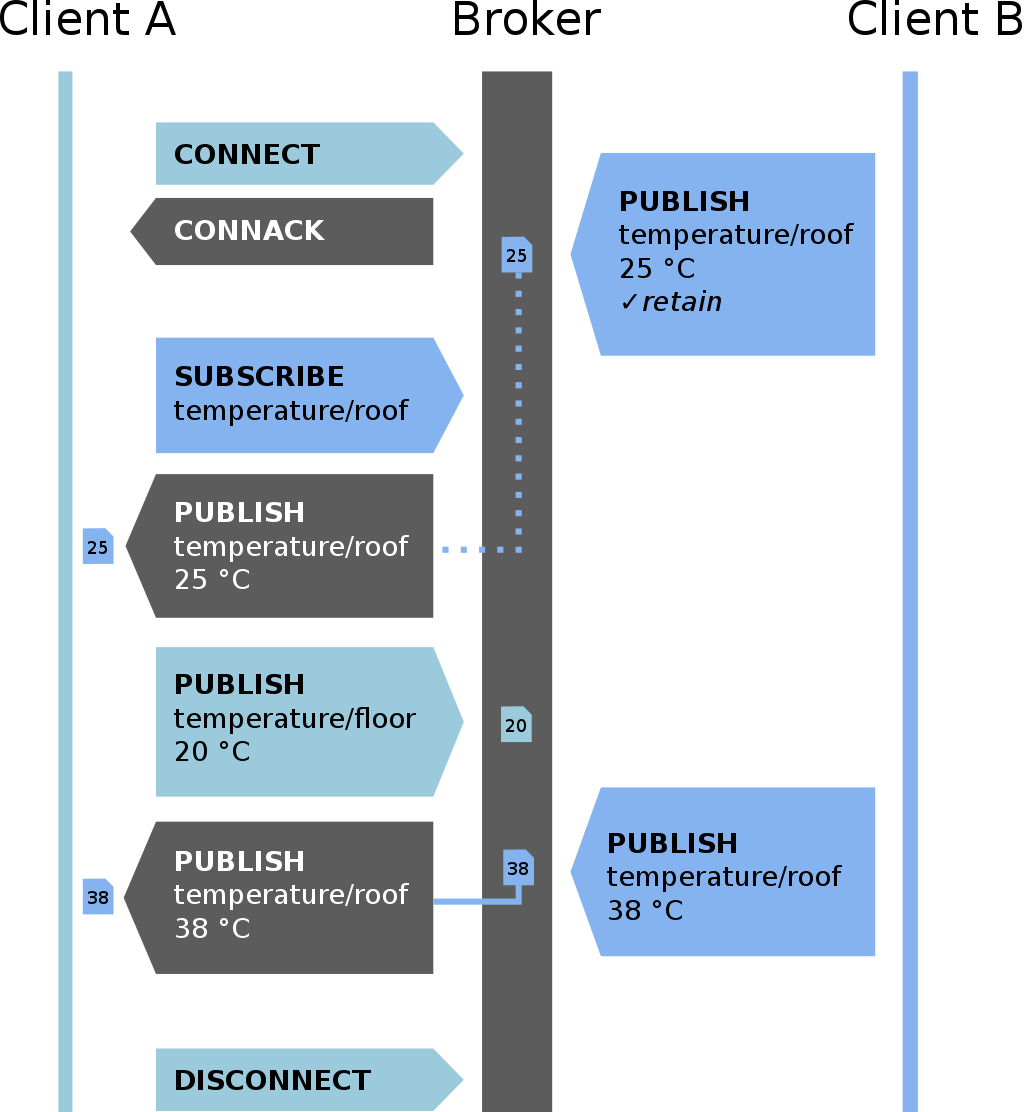
\includegraphics[width=0.8\textwidth]{img/mqtt_schematic.png}
            \caption{Schemat działania protokołu MQTT}
            \label{fig:mqtt_schematic}
        \end{figure}
         
        
    \section{Typy wiadomości}
        Istnieje obsługiwanych 14 typów wiadomości.
        
        \begin{itemize}
            \item CONNECT - Nawiązanie połączenia,
            \item CONNACK - Potwierdzenie nawiązania połączenia,
            \item PUBLISH - Publikacja wiadomości,
            \item PUBACK - Potwierdzenie publikacji wiadomości
            \item PUBREC - Potwierdzenie otrzymania wiadomości,
            \item PUBREL - Potwierdzenie wysłania wiadomości,
            \item PUBCOMP - Potwierdzenie końca publikowania wiadomości,
            \item SUBSCRIBE - Subskrypcja tematu,
            \item SUBACK - Potwierdzenie subskrypcji,
            \item UNSUBSCRIBE - Anulowanie subskrypcji,
            \item UNSUBACK - Potwierdzenie anulowania subskrypcji,
            \item PINGREQ - Żądanie PINGU,
            \item PINGRESP - Odpowiedź na żądanie PINGU,
            \item DISCONNECT - Zakończenie połączenia.
        \end{itemize}
        
        
    \section{Instalacja i konfiguracja}
        \subsection{Tworzenie kontenera}
            Instalacja brokera Mosquitto w kontenerze jest niezwykle prosta. Do uruchomienia instancji brokera wystarczy jedna komenda \ref{code:docker_install} wpisana w konsoli. W przypadku, gdy Docker nie znajdzie lokalnie danego kontenera, automatycznie pobierze on niezbędne pliki, rozpakuje je, a następnie kontynuuje uruchomienie. Jedynym wymogiem jest poprawnie przeprowadzona instalacja programu Docker.
            
            \begin{kod}
                \inputminted[lastline=2]{sh}{mqtt/listings/docker.sh}
                \caption{Utworzenie instancji brokera MQTT w kontenerze}
                \label{code:docker_install}
                \vspace{2em}
            \end{kod}
            
            Do kompleksowego zrozumienia użytego polecania warto pochylić się nad sensem wykorzystanych opcji:
            
            \begin{itemize}
                \item $run$ uruchamia nowy kontener.
                
                \item $-it$ włącza interaktywność kontenera, przekierowuje standardowy strumień wejściowy do kontenera.
                
                \item $-name$ przypisuje kontenerowi przyjazną nazwę.
                
                \item $-p$ to opcja pozwalająca przekierować port poza kontener. Domyślny port wykorzystywany przy komunikacji MQTT to 1883.
                
                \item $-v$ montowanie woluminu. W tym przypadku montowany jest on w folderze użytkownika. Taka opcja znacząco ułatwia ingerencję w pliki konfiguracyjne.
                
            \end{itemize}
            
            Na końcu polecenia znajduje się nazwa obrazu z biblioteki, który ma zostać uruchomiony.
        
        \subsection{Konfiguracja}
            Po pomyślnej instalacji wymagana jest minimalna konfiguracja programu. Plik "mosquitto.conf" jest głównym plikiem konfiguracyjnym, w którym należy zawrzeć opcje wymienione w listingu \ref{code:docker_conf}. Przede wszystkim należy ustawić wykorzystywany port na identyczny z podanym przy tworzeniu kontenera. Kolejno należy wybrać możliwość zapisywania stanów oraz ścieżkę zapisu. Ważnym aspektem jest także wymuszenie autoryzacji podczas połączenia wraz ze wskazaniem na listę dopuszczanych klientów i haseł.
            
            \begin{kod}
                \inputminted[firstline=7, lastline=11]{sh}{mqtt/listings/docker.sh}
                \caption{Minimalna konfiguracja brokera}
                \label{code:docker_conf}
                \vspace{2em}
            \end{kod}
            
        \subsection{Dodawanie użytkowników}
            Ostatnim krokiem w przygotowywaniu brokera do przyjęcia klientów jest zdefiniowanie listy akceptowanych loginów wraz z przypisanymi im hasłami. Najprostszym sposobem jest wykorzystanie dedykowanej temu celu komendy widocznej w listingu \ref{code:docker_user}.
            
            \begin{kod}
                \inputminted[firstline=14]{sh}{mqtt/listings/docker.sh}
                \caption{Dodawanie pierwszego użytkownika}
                \label{code:docker_user}
                \vspace{2em}
            \end{kod}
            
            Tworzy ona nowy plik z hasłami o nazwie $passwordfile$ jednocześnie wyzwalając inicjalizację pierwszego użytkownika o loginie $user$. Po wykonaniu polecenia zostaje wystosowane również dwukrotne zapytanie o hasło dla nowego konta.